\documentclass[11pt]{article}

\usepackage{times}
\usepackage{graphicx}

\textwidth=6.5in
\textheight=8.75in
\oddsidemargin=0.0in
\evensidemargin=0.0in
\topmargin=-0.5in

\begin{document}
\thispagestyle{empty}

\begin{center}
{\bf CS 6300} \hfill {\large\bf HW01:  Search} \hfill {\bf Due 25 January 2022}
\end{center}

Please use \LaTeX\ to produce your writeups. See the Homework Assignments 
page on the class website for details.

\section{Uninformed Search}

Consider the state space graph shown below.  A is the start state and
G is the goal state. The costs for each edge are shown on the graph.
Each edge can be traversed in both directions.

\begin{center}
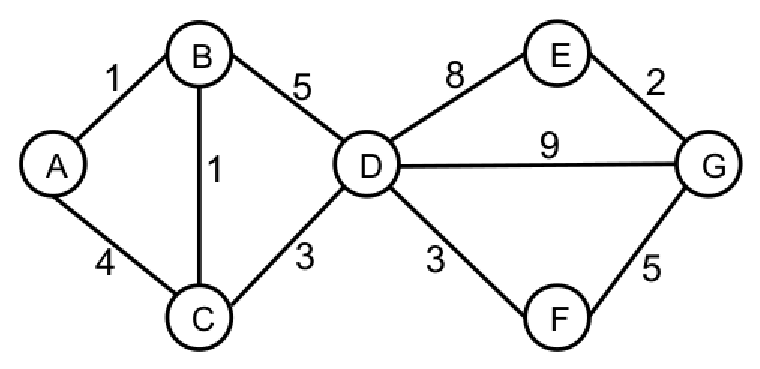
\includegraphics[width=3.5in]{search_graph.eps}
\end{center}

Execute the following search algorithms using priority queues, by
filling in the search table for each part.  (Not all steps will
necessarily be used.)

  \begin{enumerate}

  \item {\bf Breadth First Graph Search.} \\    

    \begin{center}
    \begin{tabular}{|l|l@{\hspace*{4.5in}}|l|} \hline
    \bf Step & \bf Priority Queue                                   & \bf Expand \\ \hline
    1 &                                                             &  \\ \hline
    2 &                                                             &  \\ \hline
    3 &                                                             &  \\ \hline
    4 &                                                             &  \\ \hline
    5 &                                                             &  \\ \hline
    6 &                                                             &  \\ \hline
    7 &                                                             &  \\ \hline
    8 &                                                             &  \\ \hline
    \end{tabular}
    \end{center}

\clearpage

  \item {\bf Depth First Graph Search.} \\

    \begin{center}
    \begin{tabular}{|l|l@{\hspace*{4.5in}}|l|} \hline
    \bf Step & \bf Priority Queue                                   & \bf Expand \\ \hline
    1 &                                                             &  \\ \hline
    2 &                                                             &  \\ \hline
    3 &                                                             &  \\ \hline
    4 &                                                             &  \\ \hline
    5 &                                                             &  \\ \hline
    6 &                                                             &  \\ \hline
    7 &                                                             &  \\ \hline
    8 &                                                             &  \\ \hline
    \end{tabular}
    \end{center}

  \item {\bf  Uniform Cost Graph Search.} \\

    \begin{center}
    \begin{tabular}{|l|l@{\hspace*{4.5in}}|l|} \hline
    \bf Step & \bf Priority Queue                                   & \bf Expand \\ \hline
    1 &                                                             &  \\ \hline
    2 &                                                             &  \\ \hline
    3 &                                                             &  \\ \hline
    4 &                                                             &  \\ \hline
    5 &                                                             &  \\ \hline
    6 &                                                             &  \\ \hline
    7 &                                                             &  \\ \hline
    8 &                                                             &  \\ \hline
    \end{tabular}
    \end{center}

\end{enumerate}

\clearpage

\section{Heuristic Search}

   \begin{enumerate}
  
   \item Consider the two heurisitics $h_1$ and $h_2$, only one of
     which is consistent.  Which one is consistent?

\begin{center}
\begin{tabular}{|c|c|c|c|c|c|c|c|}\hline
Node  & A   & B  & C  & D  & E   & F   & G  \\ \hline
$h_1$ & 9.5 & 9	 & 8  & 7  & 1.5 & 4   & 0  \\ \hline
$h_2$ & 10  & 12 & 10 & 8  & 1   & 4.5 & 0  \\ \hline
\end{tabular}
\end{center}

  \item Then do A* search with that heuristic.

    \begin{center}
    \begin{tabular}{|l|l@{\hspace*{4.5in}}|l|} \hline
    \bf Step & \bf Priority Queue                                   & \bf Expand \\ \hline
    1 &                                                             &  \\ \hline
    2 &                                                             &  \\ \hline
    3 &                                                             &  \\ \hline
    4 &                                                             &  \\ \hline
    5 &                                                             &  \\ \hline
    6 &                                                             &  \\ \hline
    7 &                                                             &  \\ \hline
    8 &                                                             &  \\ \hline
    \end{tabular}
    \end{center}

  \item Suppose you are completing the new heuristic function $h_3$
    shown below.  All the values are fixed except $h_3(B)$.

\begin{center}
\begin{tabular}{|c|c|c|c|c|c|c|c|}
\hline
Node & A & B & C & D & E & F & G \\
\hline
$h_3$& 10 & ?  & 9 & 7 & 1.5 & 4.5& 0 \\
\hline
\end{tabular}
\end{center}

For each of the following conditions, write the set of values that are
possible for $h_3(B)$.  For example, to denote all non-negative
numbers, write [0, $\infty$], to denote the empty set, write
$\emptyset$, and so on.

\begin{enumerate}

\item What values of $h_3(B)$ make $h_3$ admissible?

\item What values of $h_3(B)$ make $h_3$ consistent?

\item What values of $h_3(B)$ will cause A* graph search to expand
  from node A to C, then node A to B, then node A to B to D in that
  order?

\end{enumerate}

\end{enumerate}

\end{document}
